\chapter{Transverse Momentum Dependent Analysis} \label{ch::tmdanalysis}
\ifpdf
\graphicspath{{Chapters/TMDAnalysis/Figs/}}
\fi

This chapter goes over the results for two additional transverse momentum
dependent analyses from the 2015 Drell-Yan data set.  The first analysis is for
a traditional asymmetry method used at COMPASS, the double ratio method.  The
double ratio method is an analysis technique to determine spin-dependent
phenomena without acceptance effects.  The second results are from
$q_T$-weighted transverse momentum dependent asymmetries. The theoretical
introduction and motivation for measuring $q_T$-weighted asymmetries is provided
in Sec~\ref{sec::qt_w_theory}.  The author of this thesis was a cross checker
for the $q_T$-weighted asymmetry results which is a required step for any
results to become public.  For the full details of the $q_T$-weighted analysis
see reference~\cite{janthesis}.

The same data taking conditions, Sec~\ref{sec::datasample}, and stability tests,
Sec~\ref{sec::stability}, used for determining the left-right asymmetry,
Ch~\ref{ch::leftright}, are also used for both of these analyses.  In
particular, the data is from the same nine taking periods were the transversely
polarized $NH_3$ target polarization is flip between each sub-period of data
taking.  Therefore only the differences in event selection and analysis
techniques will be provided in this chapter.

\section{Double Ratio Analysis} \label{sec::doubleratio}
The double ratio method is used to determine spin-dependent asymmetry
amplitudes.  This means the asymmetry amplitudes $A^{\sin\phi_S}_T$,
$A^{\sin(2\phi+\phi_S)}_T$ and $A^{\sin(2\phi-\phi_S)}_T$ can be determined from
the 2015 transversely polarized Drell-Yan data.  The benefit of this method is
that the spectrometer acceptance does not effect the determination of the
asymmetry amplitudes.

The cuts and binning used in the left-right asymmetry analysis were determine
with the goal of determine TMD asymmetry amplitudes.  In fact, the asymmetry
amplitude $A^{\sin\phi_S}_T$ is the same amplitude as was determined in the
left-right asymmetry.  Therefore the same left-right asymmetry event selection,
Sec~\ref{sec::dy_eventselection}, and binning, Table~\ref{tab::binning}, were
also used in this analysis.

\subsection{Asymmetry Extraction}
The double ratio is defined as

\begin{equation}
  R_D(\Phi) =
  \frac{N_1^{\uparrow}(\Phi)N_2^{\uparrow}(\Phi)}
       {N_1^{\downarrow}(\Phi)N_2^{\uparrow}(\Phi)},
\end{equation}
\noindent
where the same notation is used from the left-right asymmetry notation that $N$
is the counts, 1(2) is the upstream(downstream) target and
$\uparrow$($\downarrow$) represents the transverse polarization.  The number of
counts, $N(\Phi)$, is defined as in Eq.~\ref{equ::xsection}, which when
assuming the spin-dependent Drell-Yan cross-section,
Eq.~\ref{equ::DY_MostusefulXsect}, can be written

\begin{equation}
  \label{equ::spindependentCounts}
  N(\Phi) = a(\Phi)L\sigma_U\Big(1 \pm D_{[\Phi]}|S_T|A^w_T\sin(\Phi)\Big).
\end{equation}
\noindent
Therefore the $R_D$ can be written
\begin{align}
  R_D(\Phi) &= \frac{ a_1^{\uparrow}(\Phi)L_1^{\uparrow}\sigma_U\Big(1 +
    D_{[\Phi]1}^{\uparrow}|S_{T1}^{\uparrow}|A^w_T\sin(\Phi)\Big)
    a_2^{\uparrow}(\Phi)L_2^{\uparrow}\sigma_U\Big(1 +
    D_{[\Phi]2}^{\uparrow}|S_{T2}^{\uparrow}|A^w_T\sin(\Phi)\Big) } {
    a_1^{\downarrow}(\Phi)L_1^{\downarrow}\sigma_U\Big(1 -
    D_{[\Phi]1}^{\downarrow}|S_{T1}^{\downarrow}|A^w_T\sin(\Phi)\Big)
    a_2^{\downarrow}(\Phi)L_2^{\downarrow}\sigma_U\Big(1 -
    D_{[\Phi]2}^{\downarrow}|S_{T2}^{\downarrow}|A^w_T\sin(\Phi)\Big) }
  \\ \nonumber &= \Big(\frac{a_1^{\uparrow}(\Phi)a_2^{\uparrow}(\Phi)}
     {a_1^{\downarrow}(\Phi)a_2^{\downarrow}(\Phi)} \Big)
     \Big(\frac{L_1^{\uparrow}L_2^{\uparrow}}
         {L_1^{\downarrow}L_2^{\downarrow}}\Big)
         \frac{\Big(1+D_{[\Phi]1}^{\uparrow}|S_{T1}^{\uparrow}|A^w_T\sin(\Phi)\Big)
           \Big(1+D_{[\Phi]2}^{\uparrow}|S_{T2}^{\uparrow}|A^w_T\sin(\Phi)\Big)}
              {\Big(1-D_{[\Phi]1}^{\downarrow}|S_{T1}^{\downarrow}|A^w_T\sin(\Phi)\Big)
                \Big(1-D_{[\Phi]2}^{\downarrow}|S_{T2}^{\downarrow}|A^w_T\sin(\Phi)\Big)
              }.
\end{align}
\noindent
The data is collected in two week periods where the conditions of the
spectrometer are frozen for each data taking period.  For this reason the
following reasonable acceptance assumption is made
\begin{equation}
  \label{equ::a_resonable_assump}
  \frac{a_1^\uparrow(\Phi) a_2^\uparrow(\Phi)}
       {a_1^\downarrow(\Phi) a_2^\downarrow(\Phi)}
       = C.
\end{equation}
\noindent
where $C$ is a constant.  In addition
$L^{\downarrow(\uparrow)}_2$ = $rL^{\uparrow(\downarrow)}_1$ where $r$ is a
constant reduction factor and therefore the luminosity terms cancel out as
\begin{equation}
  \frac{L_1^{\uparrow}L_2^{\uparrow}}{L_1^{\downarrow}L_2^{\downarrow}}
  = \frac{L_1^{\uparrow}rL_1^{\downarrow}}{L_1^{\downarrow}rL_1^{\uparrow}}
  = 1.
\end{equation}
\noindent
Finally the asymmetry amplitudes and target polarizations are assumed to be
small so the double ratio can be simplified to

\begin{align}
  R_D(\Phi) &=
  C\frac{\Big(1+D_{[\Phi]1}^{\uparrow}|S_{T1}^{\uparrow}|A^w_T\sin(\Phi)\Big)
    \Big(1+D_{[\Phi]2}^{\uparrow}|S_{T2}^{\uparrow}|A^w_T\sin(\Phi)\Big)}
  {\Big(1-D_{[\Phi]1}^{\downarrow}|S_{T1}^{\downarrow}|A^w_T\sin(\Phi)\Big)
    \Big(1-D_{[\Phi]2}^{\downarrow}|S_{T2}^{\downarrow}|A^w_T\sin(\Phi)\Big)}
  \\ \nonumber &\approx
  C\frac{1+\Big[D_{[\Phi]1}^{\uparrow}|S_{T1}^{\uparrow}|+D_{[\Phi]2}^{\uparrow}|S_{T2}^{\uparrow}|\Big]
    A^w_T\sin(\Phi)}
  {1-\Big[D_{[\Phi]1}^{\downarrow}|S_{T1}^{\downarrow}|+D_{[\Phi]2}^{\downarrow}|S_{T2}^{\downarrow}|\Big]
    A^w_T\sin(\Phi)} \\ \nonumber &\approx
  C\Big(1+\Big[D_{[\Phi]1}^{\uparrow}|S_{T1}^{\uparrow}|+D_{[\Phi]2}^{\uparrow}|S_{T2}^{\uparrow}|\Big]
  A^w_T\sin(\Phi)\Big)\Big(1+\Big[D_{[\Phi]1}^{\downarrow}|S_{T1}^{\downarrow}|+D_{[\Phi]2}^{\downarrow}|S_{T2}^{\downarrow}|\Big]
  A^w_T\sin(\Phi)\Big) \\ \nonumber &\approx C\Big(1 +
  \Big[D_{[\Phi]1}^{\uparrow}|S_{T1}^{\uparrow}|+D_{[\Phi]2}^{\uparrow}|S_{T2}^{\uparrow}|+D_{[\Phi]1}^{\downarrow}|S_{T1}^{\downarrow}|+D_{[\Phi]2}^{\downarrow}|S_{T2}^{\downarrow}|\Big]A^w_T\sin(\Phi)\Big).
\end{align}
\noindent
Then making the assumption that the polarizations, $S_T$, and depolarization
factors, $D_{\Phi}$ are similar, the asymmetry amplitude of interest can be
determined by fitting the double ratio with the function
\begin{equation}
  \label{equ::dr_fit_formula}
  \mathrm{fit function} = [p0](1+4[p1]\sin(\Phi),
\end{equation}
\noindent
where $[p0]$ and $[p1]$ are fit parameters and $[p1]$ represents the asymmetry
amplitude of interest.  The $[p1]$ parameter is later corrected for polarization
and depolarization factors.

The double ratio, $R_D$, is determine as a function of $\Phi$ where the angle
$\Phi$ depends on which asymmetry amplitude is being determined.  The assumption
made in the measured counts formula, Eq.~\ref{equ::spindependentCounts}, is that
all angles except the spin-dependent $\Phi$ angle are integrated over.  When
this is the true, all the other fourier components, except the constant term,
from the Drell-Yan cross-section, Eq.~\ref{equ::DY_MostusefulXsect}, integrate
to zero.  The following table, Table~\ref{tab::ratio_phiAngles}, list which
$\Phi$ angle is used to determine which spin-dependent asymmetry amplitude.

\begin{table}[h!t]
  \centering
  \caption{Measured counts as a function of each $\Phi$ angle}
  \begin{tabular}{ |c|c|c|c| }
    \hline \textbf{Asymmetry Amplitude}& \textbf{Corresponding TMD Function}&
    \textbf{$\Phi$ Angle}& \textbf{$\Phi$ Range (radians)} \\ \hline
    
    $A^{\sin(\phi_S)}_T$& Sivers& $\phi_S$& [-$\pi$, $\pi$] \\ \hline

    $A^{\sin(2\phi-\phi_S)}_T$& Transversity& $2\phi-\phi_S$& [-3$\pi$, 3$\pi$]
    \\ \hline

    $A^{\sin(2\phi+\phi_S)}_T$& Preztelosity& $2\phi+\phi_S$& [-3$\pi$, 3$\pi$]
    \\ \hline
  \end{tabular}
    \label{tab::ratio_phiAngles}
\end{table}

The variance of the double ratio, assuming Poisson counting statistics, is

\begin{equation}
  \sigma^2_{R_D} = R^2_D(\Phi)\Big(\frac{1}{N_1^\uparrow(\Phi)}
    + \frac{1}{N_2^\uparrow(\Phi)}
    + \frac{1}{N_1^\downarrow(\Phi)}
    +\frac{1}{N_2^\downarrow(\Phi)}
   \Big).
\end{equation}

\subsection{Results}\label{sec::doubleratio_results}
The results of each asymmetry amplitude are determined in each of the nine
periods and combined using the weighted average as in Eq.~\ref{equ::wAvg}.  For
each period and each kinematical bin, the asymmetry is determined by fitting the
double ratio and with Eq.~\ref{equ::dr_fit_formula}.  The results of the fit
actually determine the value

\begin{equation}
  A^w_T \langle D_{[\Phi]} \rangle \langle |S_T|\rangle.
\end{equation}
\noindent
The asymmetry amplitude is finally determined by dividing the fit results by the
average polarization and depolarization values per period.

To determine the asymmetry amplitude, the double ratio is binned in eight bins
in $\Phi$.  Eight bins are chosen due to the low statistics from Drell-Yan data.
Fig.~\ref{fig::dr_exmaple_trans} shows an example of the binned double ratio and
a fit.

\begin{figure}[h!t]
  \centering 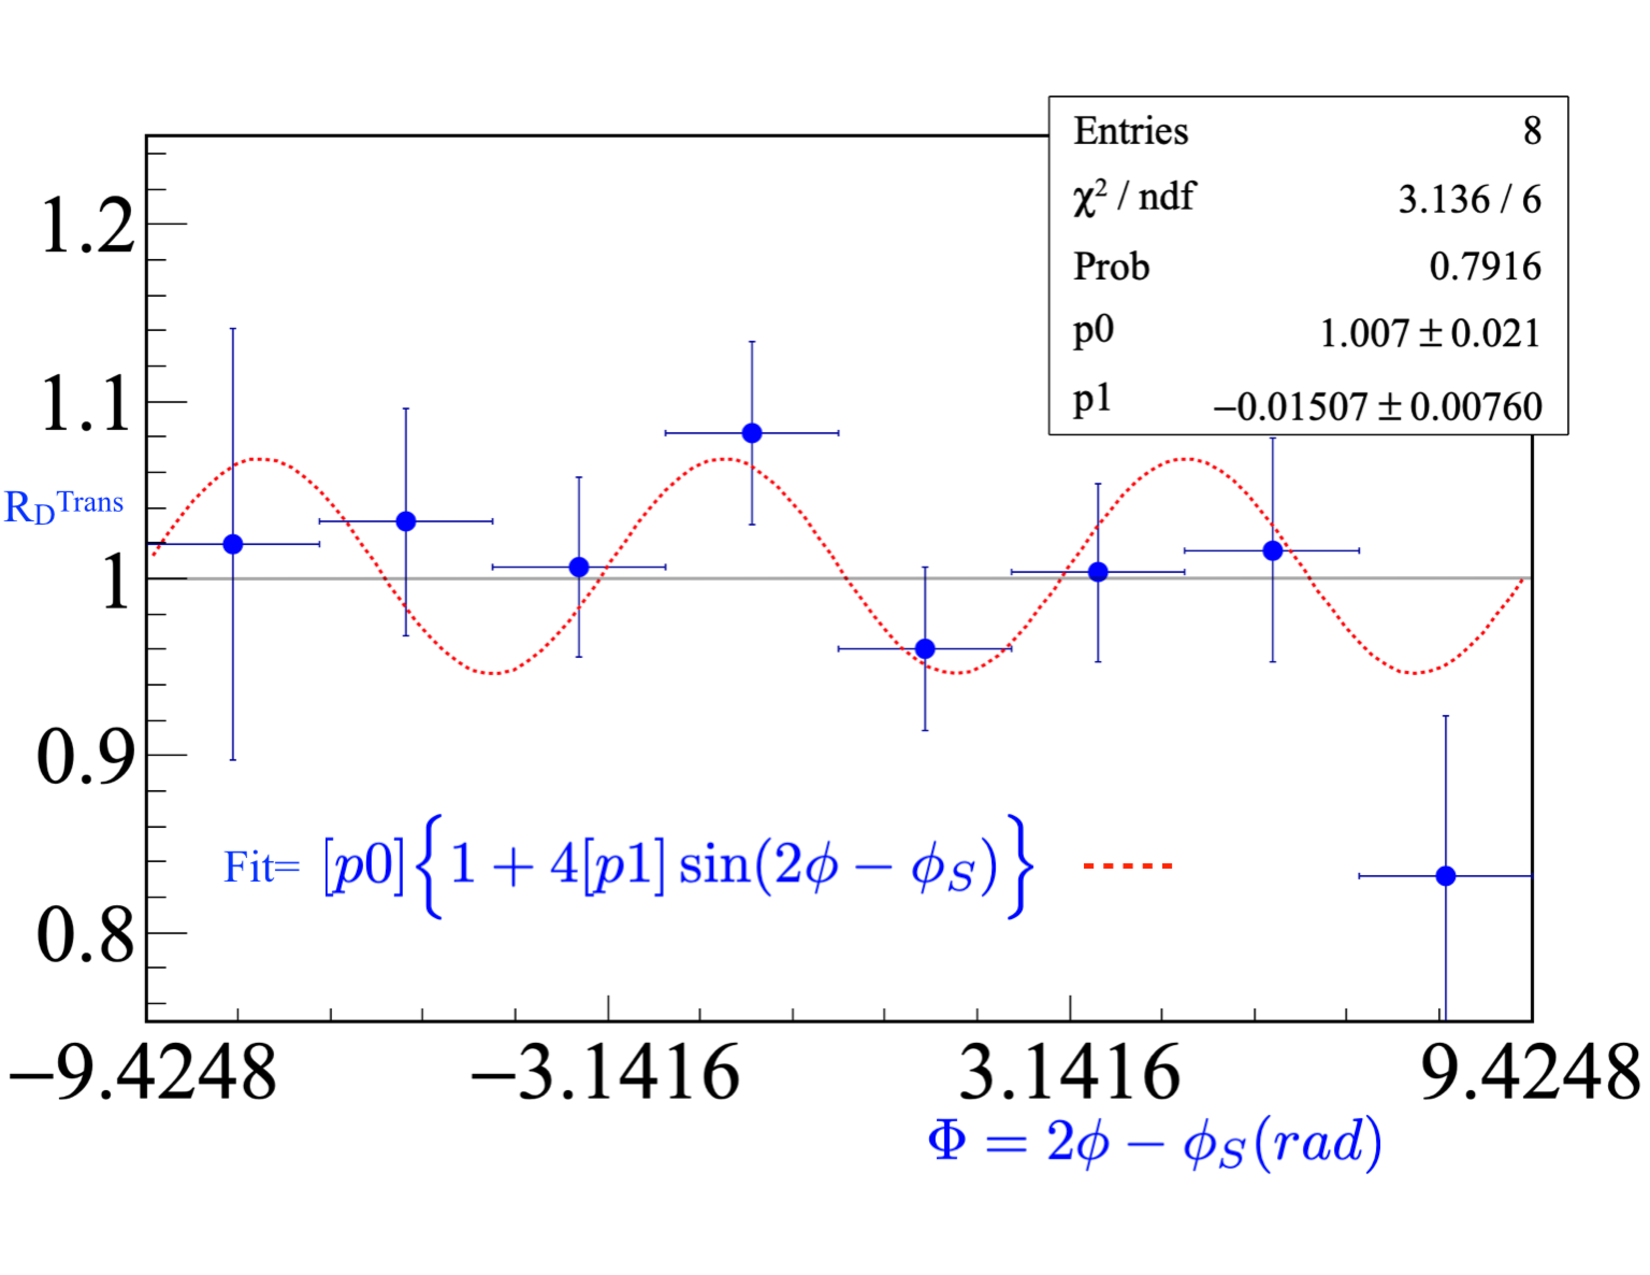
\includegraphics[width=0.6\textwidth,trim=0cm 1cm 0cm 1cm,
    clip]{dr_example_trans}
  \caption{An example double ratio and corresponding fit (red) to determine the
    amplitude $A_T^{\sin(2\phi-\phi_S)}$}
  \label{fig::dr_example_trans}
\end{figure}

\noindent
The results for all the spin-dependent asymmetry amplitudes are show in
Fig.~\ref{fig::dr_final_results}.  As can be seen, the significance of the
integrated asymmetry amplitudes is: over 1 sigma above zero for the Sivers,
$A^{\sin\phi_S}_T$, over 3 sigma above zero for Preztelosity,
$A^{\sin(2\phi+\phi_S)}_T$, and 3 sigma below zero for transversity,
$A^{\sin(2\phi-\phi_S)}_T$.

\begin{figure}[h!t]
  \centering 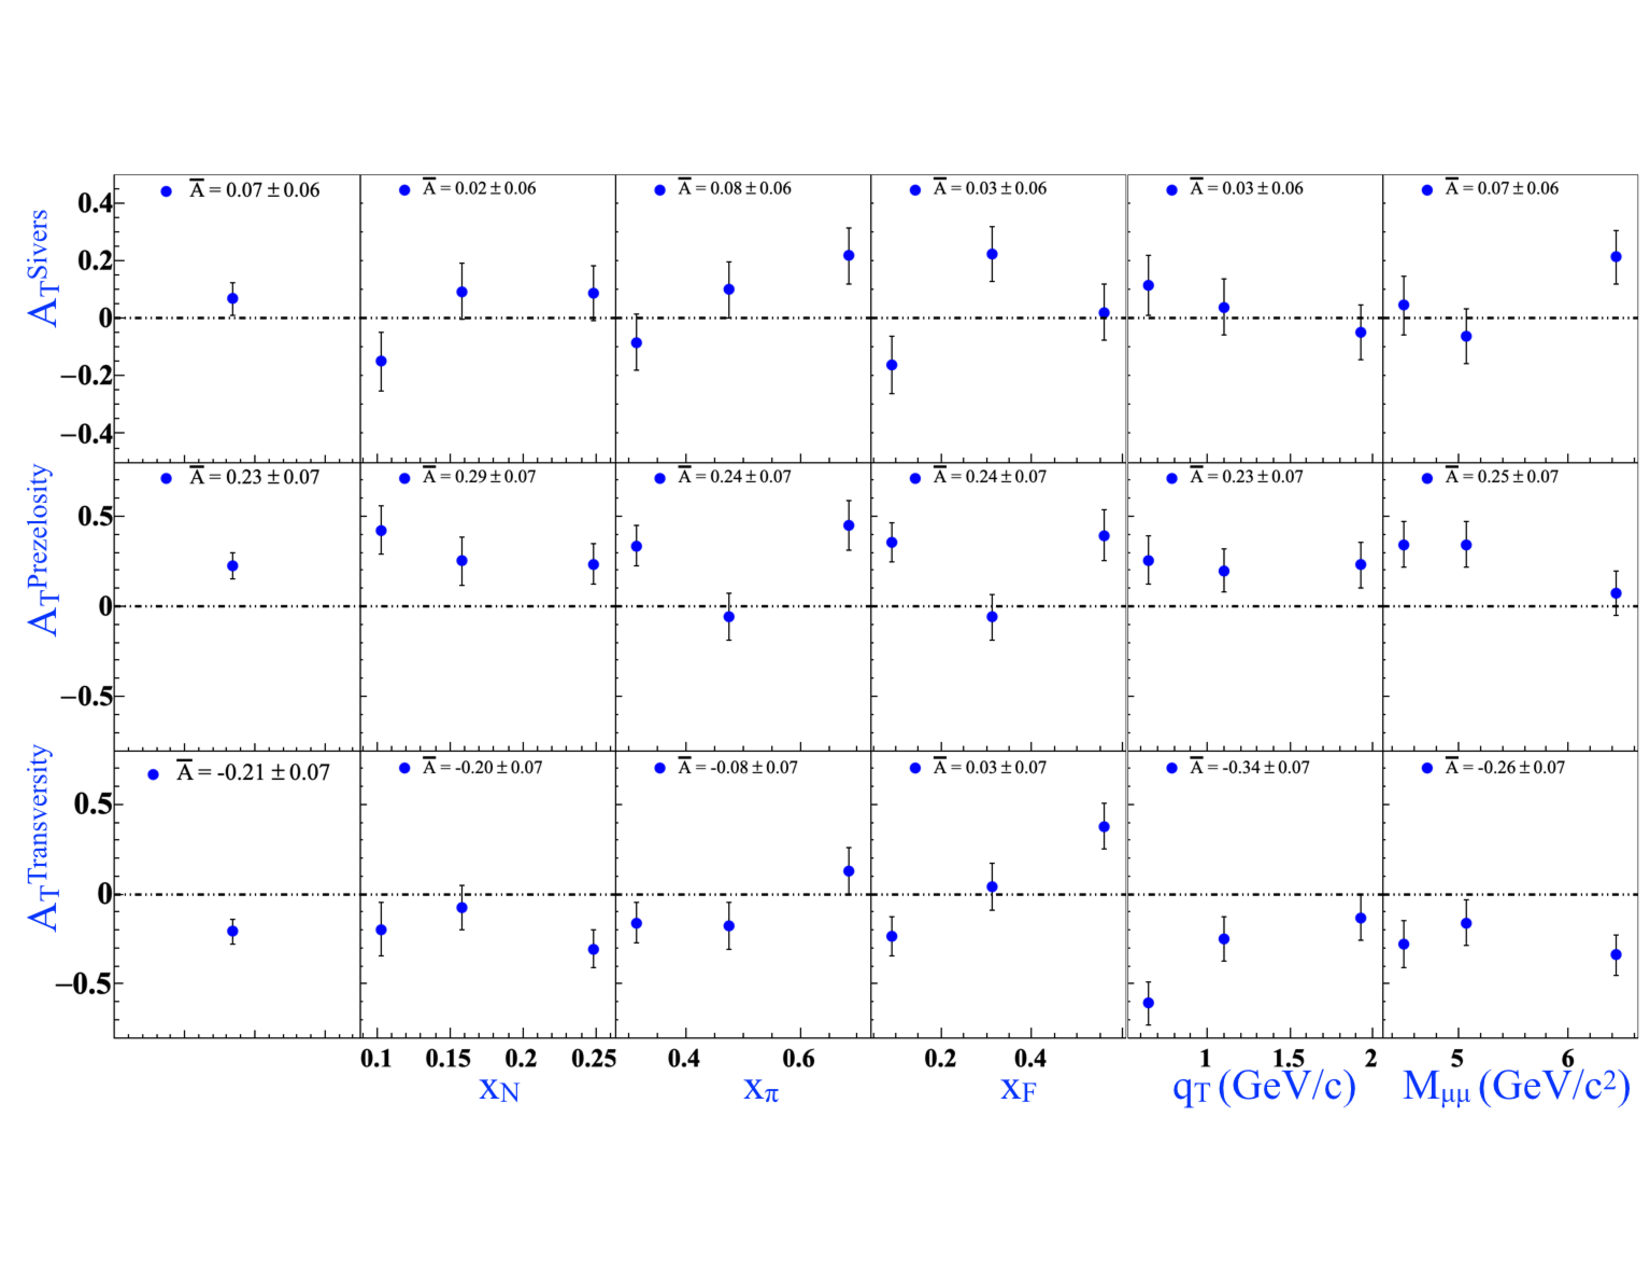
\includegraphics[width=\textwidth,trim=0cm 2.5cm 0cm 3cm,
    clip]{dr_final_results}
  \caption{The results and statistical error bars for the transverse
    spin-dependent asymmetry amplitudes $A^{\sin\phi_S}_T$ (top),
    $A^{\sin(2\phi+\phi_S)}_T$ (middle) and $A^{\sin(2\phi-\phi_S)}_T$ (bottom)
    determined from the double ratio method.}
  \label{fig::dr_final_results}
\end{figure}

to compare with the results from the TSA analysis
Include TSA results for comparisons


\section{$q_T$-Weighted Asymmetries} \label{sec::qtweighted}

The $q_T$ weighting asymmetries analysis is used to determine three asymmetry
amplitudes related to TMD functions.  This analysis determined the three
amplitudes: $A_T^{\sin(\phi_S) q_T/M_N}$, $A_T^{\sin(2\phi+\phi_S)
  q^3_T/(2M_{\pi}M_N^2)}$ and $A_T^{\sin(2\phi-\phi_S) q_T/M_{\pi}}$ which are
related to the Sivers, Preztelosity and transversity TMD PDFs respectively.

\subsection{Event Selection}
The results for this analysis were released prior to the slot1 reconstruction
production and therefore this analysis uses the t3 reconstruction.  For
$q_T$-weighted asymmetries the results depend on the full range of the $q_T$
distribution.  In the analysis of the left-right asymmetry however, a cut was
placed on high and low $q_T$ values to ensure better azimuthal angular
resolution and quality reconstructed events.  This cut cannot be applied for
$q_T$-weighted analysis because it will effect the weighting used to determine
the asymmetry.  On the other hand the high $q_T$ events from combinatorial
background and badly reconstructed events should be cut.  The next section goes
into the details and the remedy for a $q_T$ related cut. All of the other cuts
from Sec~\ref{sec::dy_eventselection} are the same except for this $q_T$
cut. Table~\ref{tab::qt_EventTable} provides the final cut order and the
remaining statistics after each cut.

\subsubsection{High $q_T$} \label{sec::high_qt}
For both the left-right asymmetry analysis and the double ratio analysis the
event selection includes a cut limiting $q_T\; < \;5\; GeV/c$ to ensure quality
of the reconstructed events.  Higher $q_T$ events are often unphysical results
from bad reconstruction or combinatorial background events.  The $q_T$
distribution without any $q_T$ cuts is shown in Fig.~\ref{fig::qT_noCuts} and as
can be seen the $q_T$ distribution reaches values much higher than 5~{\gvc}.
The most fundamental problem with this $q_T$ distribution is that some of the
events violate conservation of momentum.  A first remedy to the high $q_T$
values then is to add a cut which demands momentum conservation.  This is
achieved by demanding that the momentum sum of the detected muons is physically
possible which means $\ell^+ \; + \; \ell^- \; < \; 190$~GeV/c.  Note that this
cut does not take into account the momentum spread of the beam due to the fact
that the beam momentum spread is expected to be small.
Fig.~\ref{fig::qT_PconserveCut} shows how this cut effects the $q_T$
distribution.  As can be seen, $q_T$ still reach values much higher than the 5
GeV/c cut from the other TMD analyses.  The remaining high $q_T$ events still
have the potential to be poorly reconstructed events or combinatorial background
and for this reason an additional cut was put on the individual muons transverse
momentum so that $\ell_T^{\pm} \; <$ 7 GeV/c.

\begin{figure}[h!t]
  \centering
  \begin{subfigure}{.46\textwidth}
    \centering 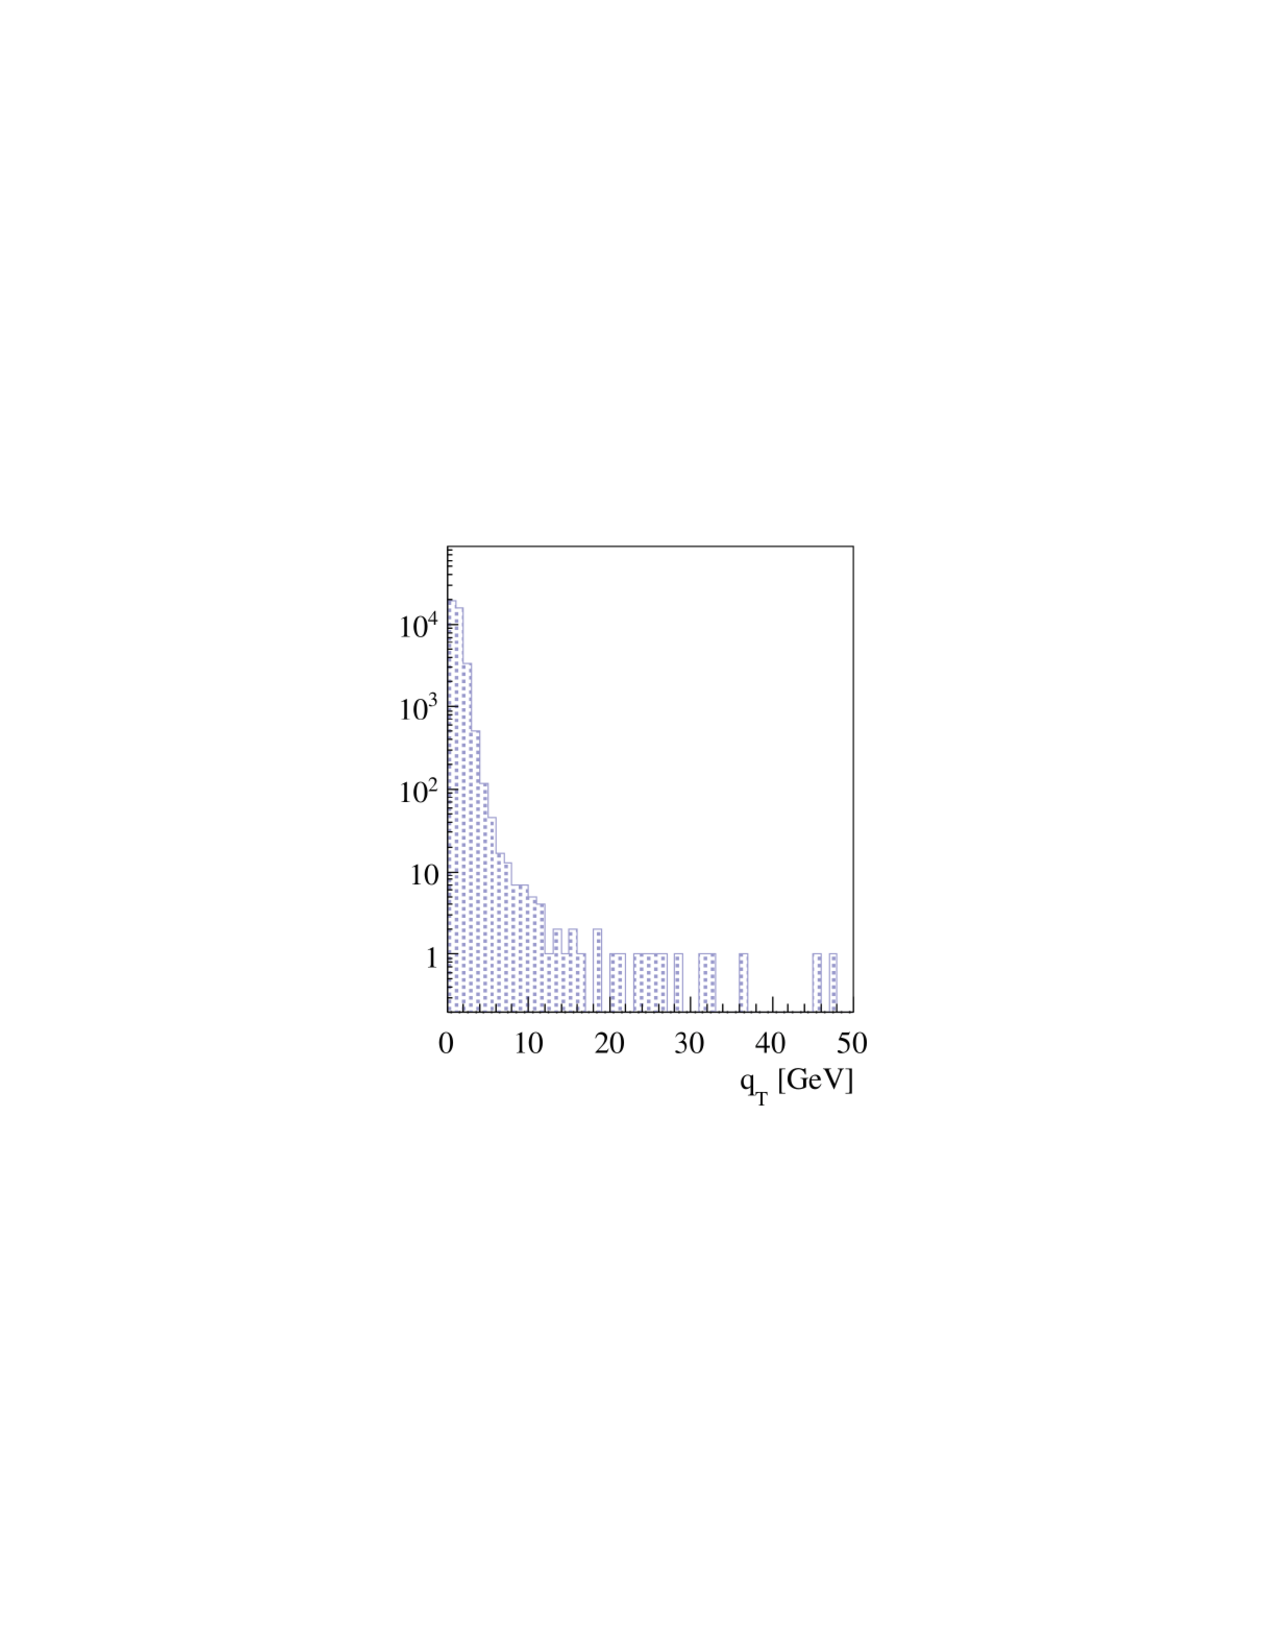
\includegraphics[width=\linewidth, trim=6cm 8.7cm 6cm 8cm,
      clip]{qT_noCuts}
    \caption{$q_T$ distribution without cuts on $q_T$.  All other cuts expect
      the $q_T$ cut from table~\ref{tab::cutdescrip} are applied.  This image is
      from~\cite{janthesis}}
    \label{fig::qT_noCuts}
  \end{subfigure}%
  \begin{subfigure}{.02\textwidth}
    \centering
    
\includegraphics[width=\linewidth]{tmp2}
    \label{fig::tmp2}%
  \end{subfigure}
  \begin{subfigure}{.46\textwidth}
    \centering 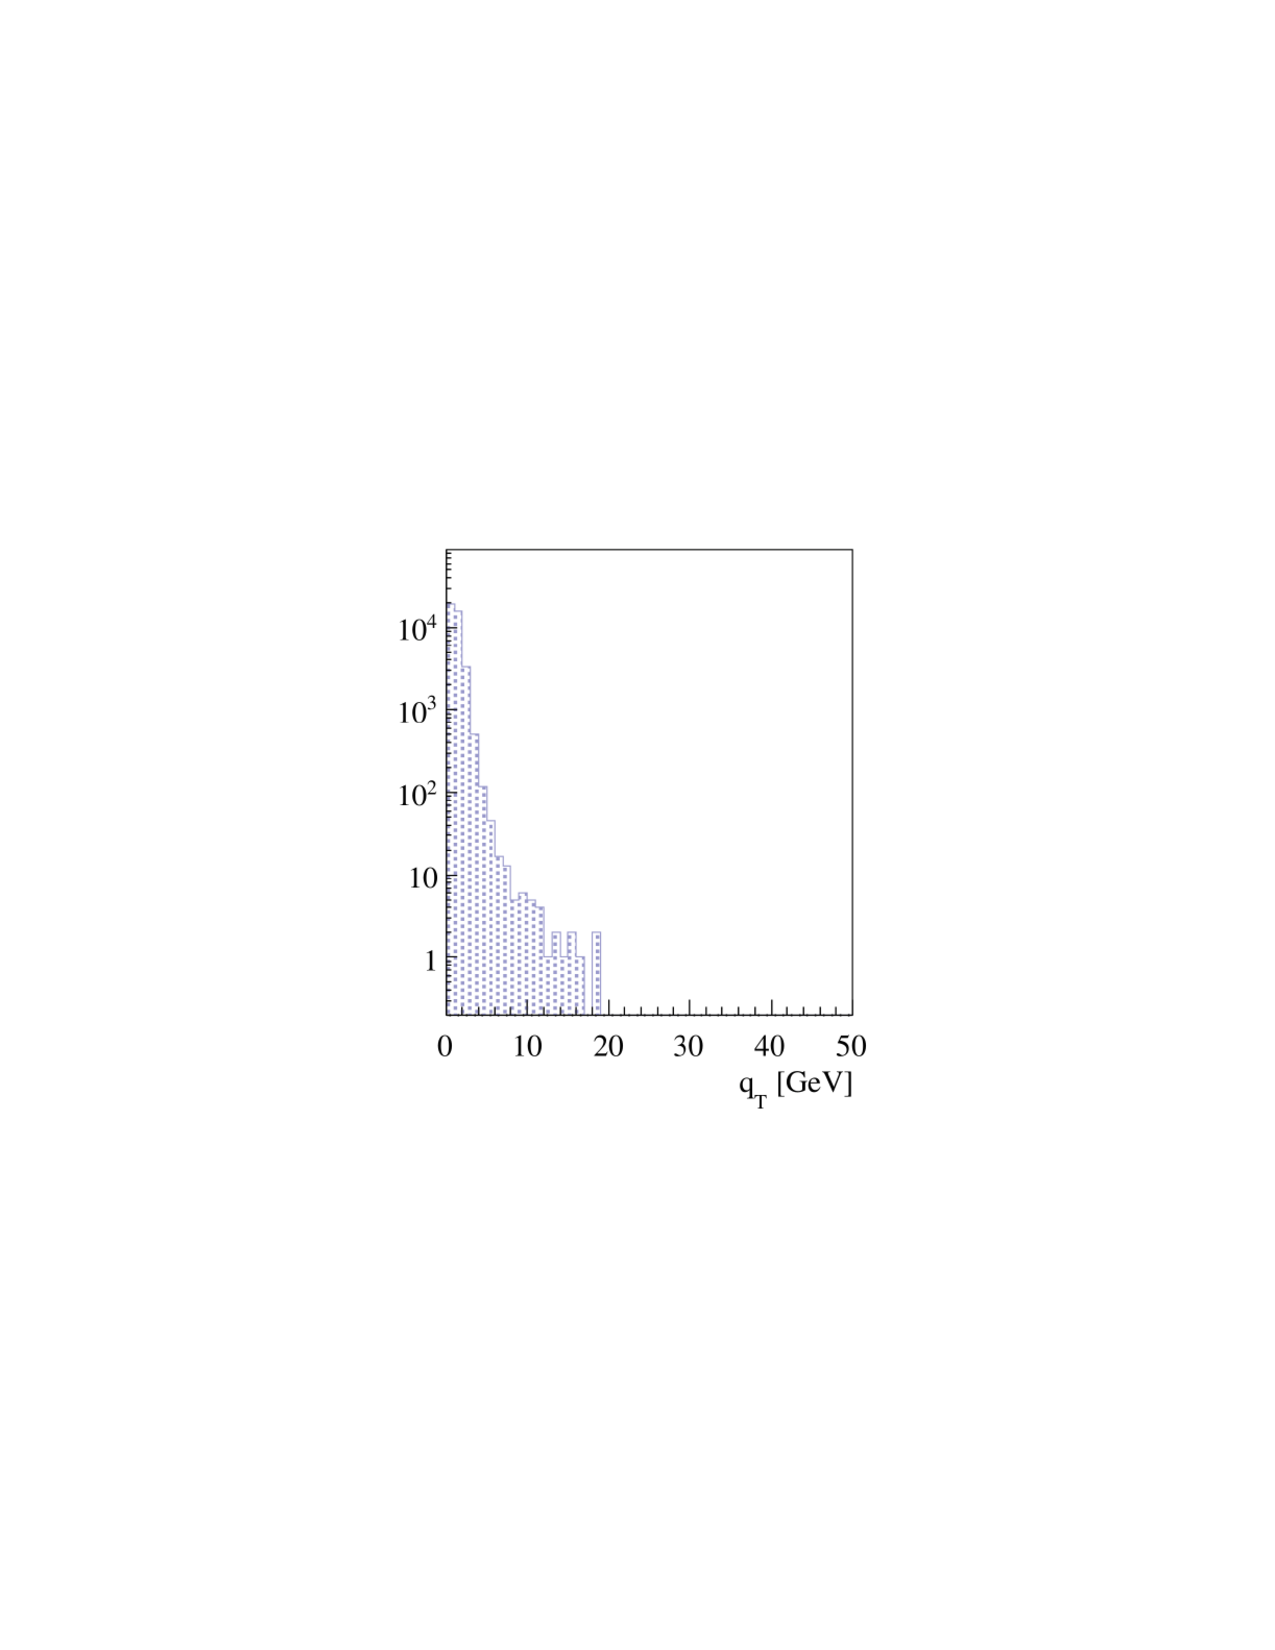
\includegraphics[width=\linewidth, trim=6cm 9cm 6cm 8cm,
      clip]{qT_PconserveCut}
    \caption{$q_T$ distribution after the momentum conservation cut is added,
      $\ell^+ \; + \; \ell^- \; < \; 190$ GeV/c.  All other cuts expect the
      $q_T$ cut from table~\ref{tab::cutdescrip} are applied.  This image is
      from~\cite{janthesis}}
    \label{fig::qT_PconserveCut}
  \end{subfigure}
\end{figure}

\begin{figure}[h!t]
  \centering
    \begin{tabular}{ |c|c|c| }
      \hline \textbf{Cuts}& \textbf{Events} & \textbf{\% Remaining} \\ \hline

      \multirow{2}{15em}{$\mu^+\mu^-$ from best primary vertex,
        4.3$<M_{\mu\mu}<8.5$ GeV/c$^2$}& 1,159,349& 100.00\\ & & \\ \hline
      
      \multirow{2}{14em}{Triggers: (2LAS or LASxOT) and not LASxMiddle}& 
      868,291& 74.89\\ & & \\ \hline
      
      Z$_{first} <$ 300 cm, Z$_{last} >$ 1500 cm& 784,379& 67.66\\ \hline

      $\Delta$t defined& 776,643& 66.99\\ \hline
      
      $|\Delta\mathrm{t}| <$ 5 ns& 337,081& 32.18\\ \hline

      $\chi^2_{track}$/ndf $<$ 10& 370,054& 31.92\\ \hline

      $\ell^+ + \ell^- < 190$ GeV/c& 219,304& 18.92\\ \hline

      $\ell_T^\pm < 7$ GeV/c& 219,014& 18.89\\ \hline

      Trigger Validation& 168,939& 14.57\\ \hline

      Good Spills& 137,812& 11.89\\ \hline

      0$<$ x$_{\pi}$ x$_N$ $<$1, -1$<$ x$_F$ $<$1& 137,802& 11.89  \\ \hline

      Z Vertex within NH$_3$& 42,646& 3.68\\ \hline

      Vertex Radius $<$ 1.9cm& 39,088& 3.37\\ \hline

    \end{tabular}
    \caption{Event selection statistics for $q_T$-weighed asymmetry analysis
      from all periods combined}
    \label{tab::qt_EventTable}
\end{figure}

\subsection{Binning}
The asymmetry is determined in bins of the Drell-Yan physical kinematic
variables: $x_N$, $x_\pi$, $x_F$ and $M_{\mu\mu}$ and an overall integrated
value.  No $q_T$ binning is used because a full integrated of the $q_T$ variable
needs to be taken into account to form the weighted asymmetry.  The binning
boundaries and bin centers for the physical kinematics are the same as that of
the left-right asymmetry and are provided in Tab~\ref{tab::binning}.

\subsection{Asymmetry Method}
The weighted asymmetry amplitudes $A_T^{\sin(\phi_S) q_T/M_N}$,
$A_T^{\sin(2\phi+\phi_S) q^3_T/(2M_{\pi}M_N^2)}$ and $A_T^{\sin(2\phi-\phi_S)
  q_T/M_{\pi}}$ are all determined using a modified double ratio.  As with the
double ratio method from Sec~\ref{sec::doubleratio}, the modified double ratio
does not depend on the spectrometer acceptance.  The modified double ratio is
defined as

\begin{equation}
  \label{equ::modified_dr}
  R^W_{DM}(\Phi)=
  \frac{N^{\uparrow W}_{1}N^{\uparrow W}_{2}
    - N^{\downarrow W}_{1}N^{\downarrow W}_{2}}
       {\sqrt{(N^{\uparrow W}_{1}N^{\uparrow W}_{2}
         + N^{\downarrow W}_{1}N^{\downarrow W}_{2})
         (N^{\uparrow}_{1}N^{\uparrow}_{2}
         + N^{\downarrow}_{1}N^{\downarrow}_{2})}},
\end{equation}
\noindent
where similar notation is used from the previous analyses where
$\uparrow$($\downarrow$) is the transverse polarization direction, 1(2) denotes
the upstream(downstream) cell, $N^{W}$ is the weighted counts, $W$ is the weight
used and $N$ denotes the unweighted counts.  The angles $\Phi$, in the modified
double ratio, are the same used for the double ratio,
Table~\ref{tab::ratio_phiAngles}, and give access to asymmetry amplitudes
related to the same corresponding TMD functions.  Under the same reasonable
acceptance ratio assumption, Eq.~\ref{equ::a_resonable_assump}, from the double
ratio method the acceptance cancels out in the double ratio method.  Using this
assumption, the modified double ratio reduces to

\begin{equation}
  \label{equ::dr_fit_form}
  R^W_{DM}(\Phi) \approx 2 \tilde{D}_{\sin\Phi}\langle S_T \rangle
  A_T^{\sin(\Phi)W} \sin\Phi,
\end{equation}
\noindent
where $\tilde{D}_{\sin\Phi}$ is an integrated depolarization factor defined as

\begin{equation}
  \tilde{D}_{\sin\phi_S} = 1, \quad\quad \tilde{D}_{\sin(2\phi\pm\phi_S)} =
  \frac{\int a(\theta)\sin^2\theta d\cos\theta} {\int a(\theta)(1+\cos^2\theta)
    d\cos\theta} = \frac{1-\langle \cos^2\theta\rangle} {1+\langle
    \cos^2\theta\rangle}.
\end{equation}

The statistical error for the modified double ratio is

\begin{equation}
  \sigma^2_{R^W_{DM}} = \frac{\sum_{c,p} \sigma^2_{N_c^{pW}}
    4(N^{\uparrow}_1N^{\uparrow}_2)N^{\downarrow}_1N^{\downarrow}_2)^2}
        {\sum_{c,p} \sigma^2_{N_c^{p}}
          (N^{\uparrow}_1N^{\uparrow}_2 + N^{\downarrow}_1N^{\downarrow}_2)^4}
        \sum_{c,p}\frac{1}{N_c^p},
\end{equation}
\noindent
where $\sigma^2_{N_c^{pW}} = \sum (W^p_c)^2$ is the sum of event weights, $c$ is
cell 1 or cell 2 and $p$ is polarization $\uparrow$ or $\downarrow$.

The weighted asymmetry amplitude are determined by forming the modified double
ratio in eight bins in the appropriate $\Phi$ angle and fitting this
distribution.  If an infinite number of bins where used with sufficient data,
the modified double ratio would be the function form of
Eq.~\ref{equ::dr_fit_form}.  $R^W_{DM}$ is binned in eight bins due to the
limited statistics.  To account for the fact that ratio is determined in a
finite number of $\Phi$ bins, the average value of Eq.~\ref{equ::dr_fit_form}
over the bin width is used as the fit distribution.  This means the functional
fit is

\begin{equation}
  \langle R^W_{DM} \rangle = \frac{1}{\Delta\Phi}
  \int_{\Phi_i-\frac{\Delta\Phi}{2}}^{\Phi_i+\frac{\Delta\Phi}{2}} R^W_{DM}
  d\Phi = \frac{2}{\Delta\Phi}\sin(\frac{\Delta\Phi}{2})R^W_{DM}(\Phi_i),
\end{equation}
\noindent
where $\Delta\Phi$ = $\frac{2\pi}{8}$ for eight bins in $\Phi$.
Fig.~\ref{fig::DRFitSiv} shows the double ratio as a function of $\Phi=\phi_S$
for period W07 in one bin of $x_N$.  One $R^W_{DM}$ is determined for each of
the 3 (number of bins) $\times$ 9 (number of periods) $\times$ 3 (number of
asymmetry amplitudes) = 81 modified double ratios.

\begin{figure}[h!t]
  \centering 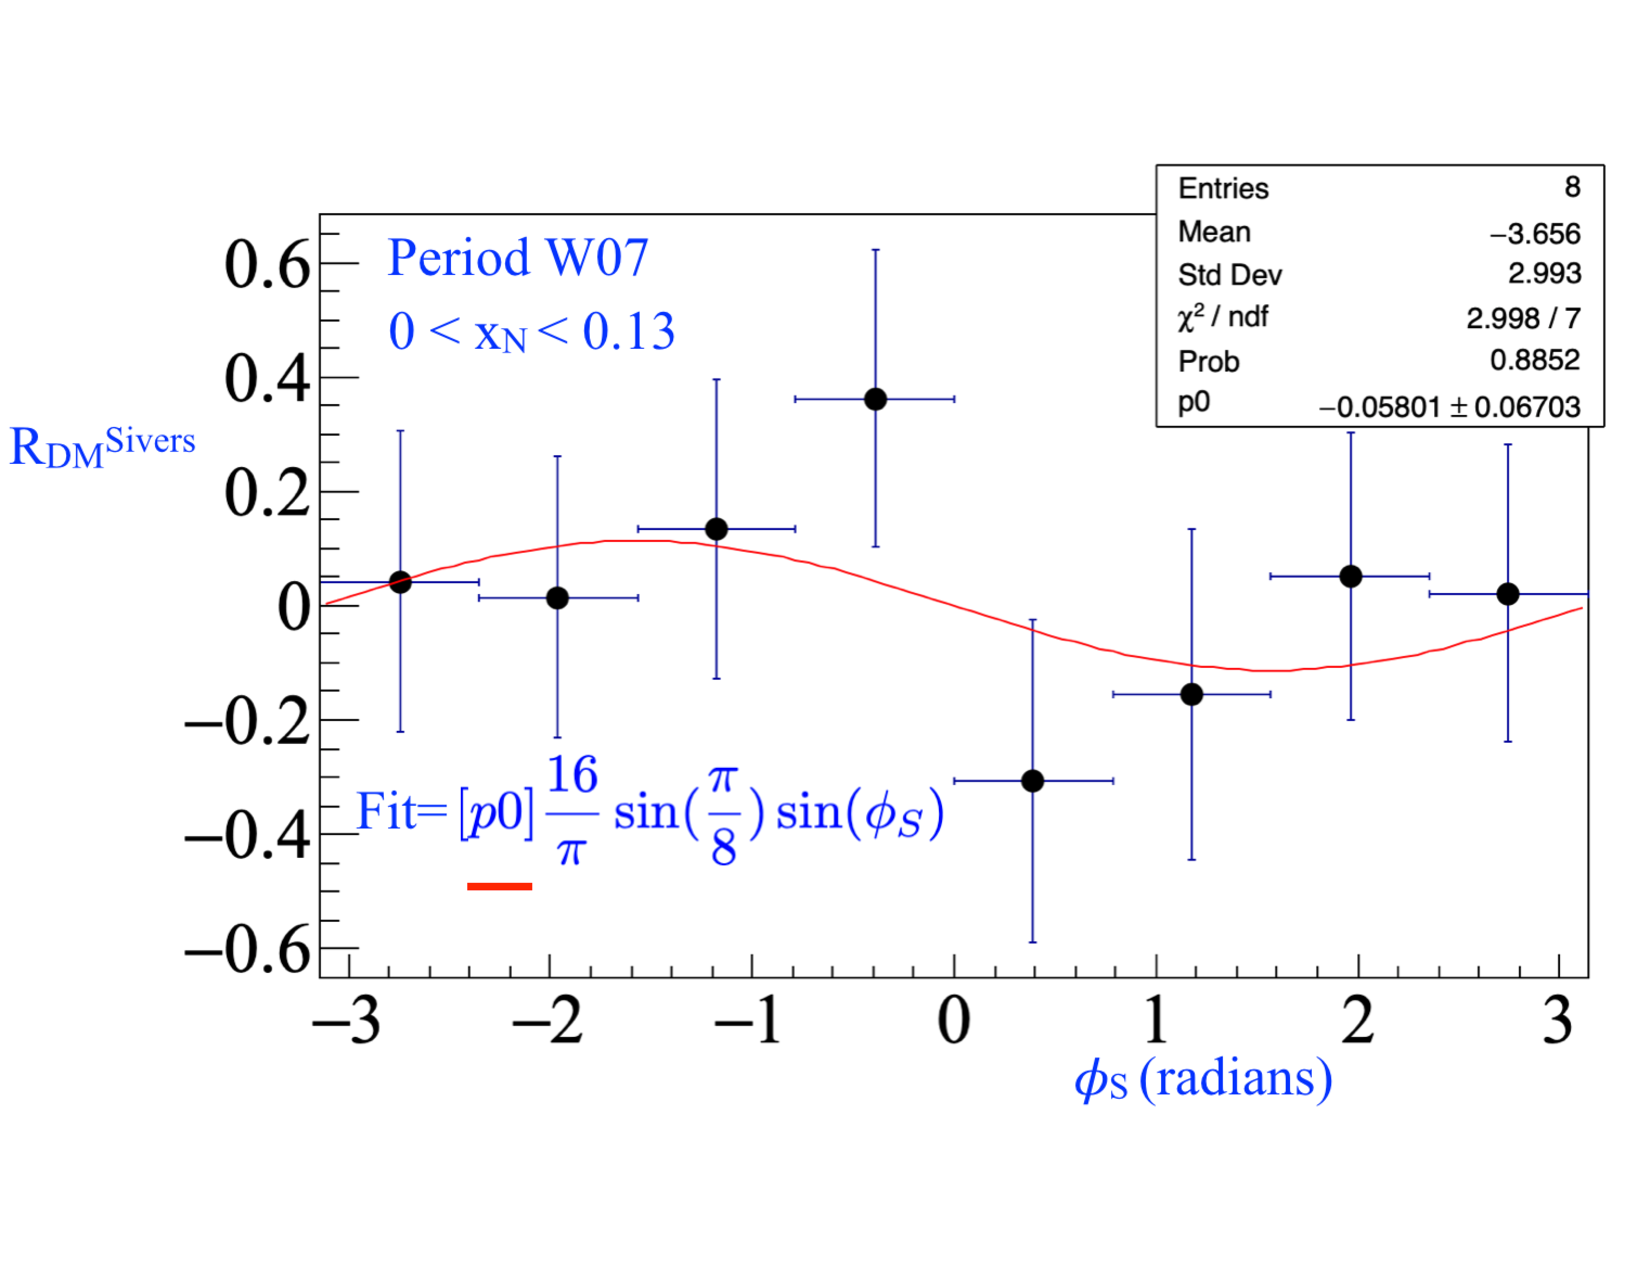
\includegraphics[width=0.6\textwidth, trim=0cm 2.5cm 0cm
    2.5cm,clip]{DRFitSiv}
  \caption{The double ratio as a function of $\phi_S$ used to determine the
    Sivers asymmetry amplitude.  This is for period W07 and the lowest bin in
    $x_N$.  The red line shows the fit and the results of the fit are shown in
    the statistics box.}
  \label{fig::DRFitSiv}
\end{figure}

\subsection{Results}
As with the other analyses in this thesis, the asymmetry amplitudes are
determine for each period and the final asymmetry is determined as a period
weighted average as in Eq.~\ref{equ::wAvg}.  For the same reason as the previous
analyses and explained in Sec~\ref{sec::doubleratio_results}, the polarization
and depolarization factors from each period are used to correct the asymmetry
amplitude determined in each period.  The final results are shown in
Fig.~\ref{fig::wA_results} along with the results from the release values.  As
can be seen the results agree with those results obtained for the release which
was a requirement before the results could be release to the public.

\begin{figure}[h!t]
  \centering 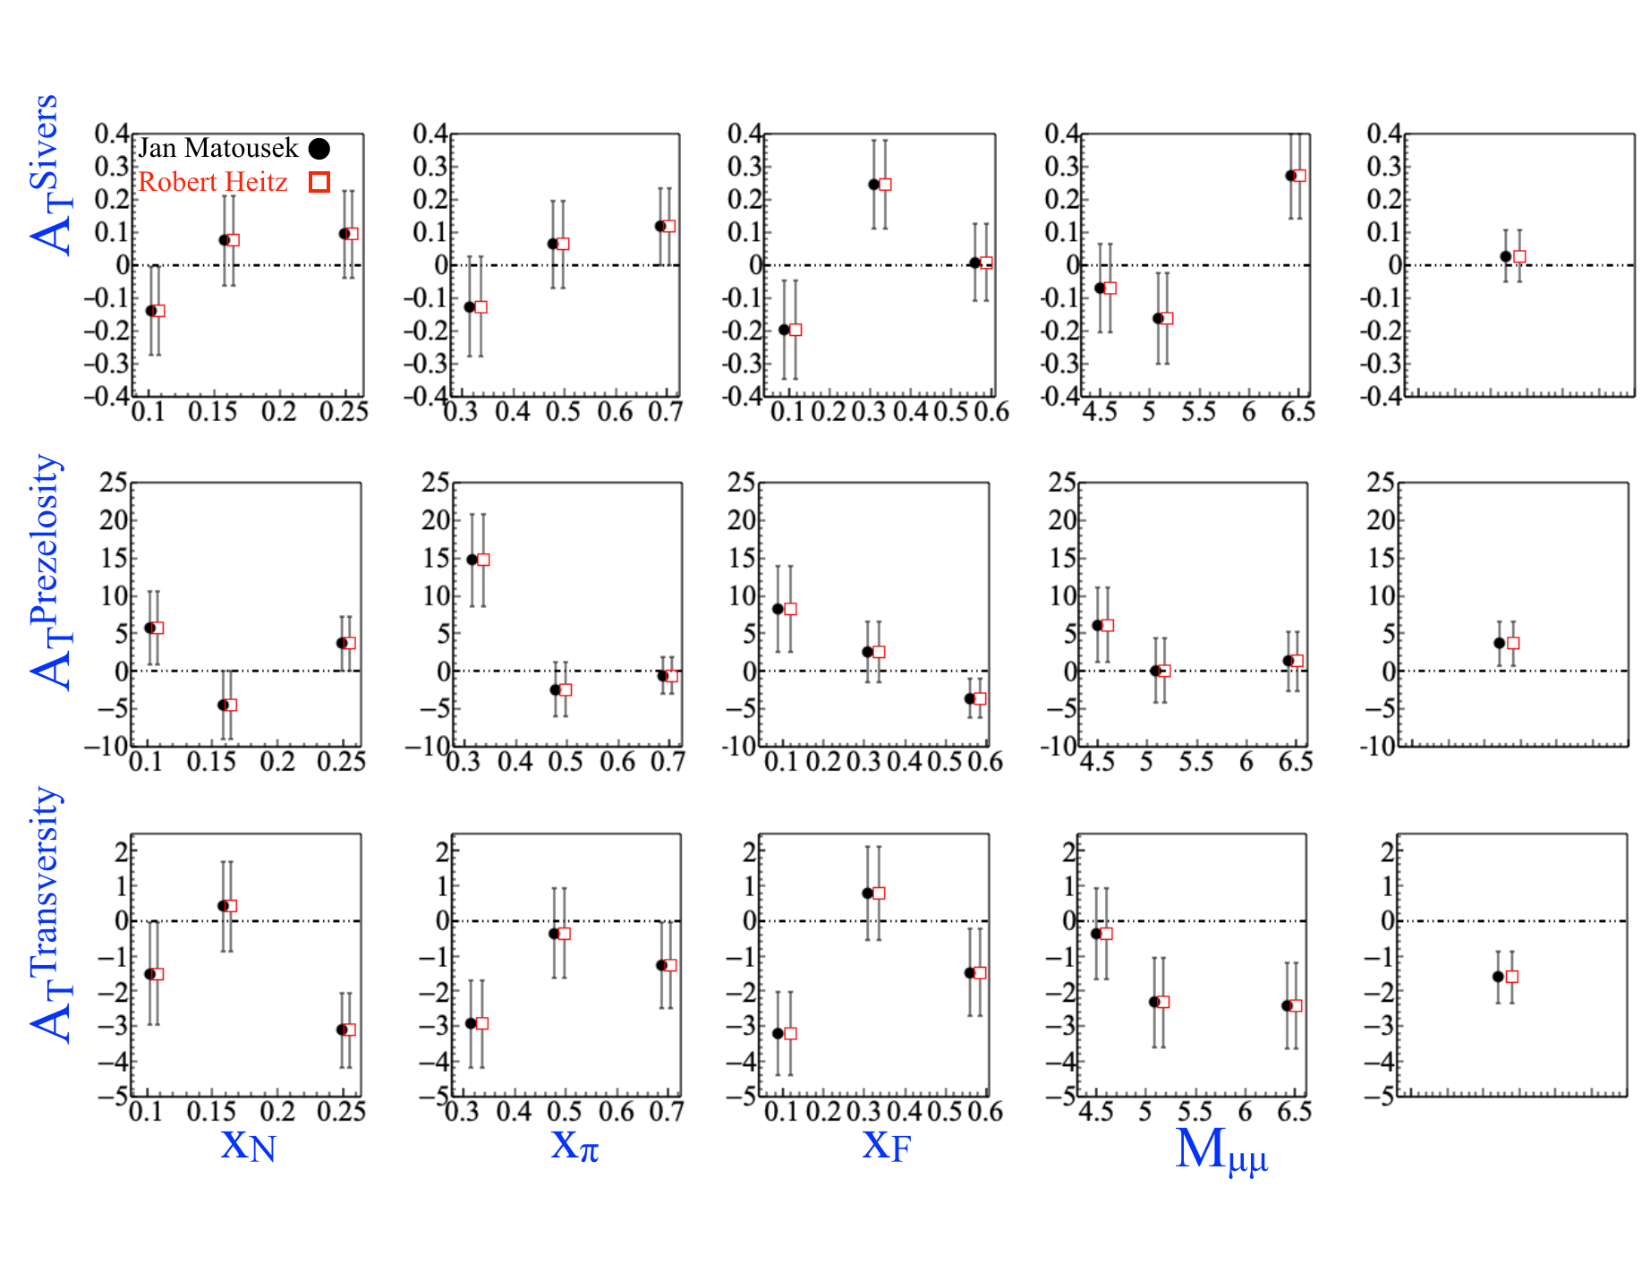
\includegraphics[width=\textwidth,trim=0.2cm 1.5cm 0.2cm 1.5cm,
    clip]{wA_results}
  \caption{The comparison of weighted asymmetry amplitude results from the
    released values from Jan Matousek (black) and the cross checker Robert Heitz
    (red).  From the top row down the asymmetry amplitudes are
    $A_T^{\sin(\phi_S) q_T/M_N}$, $A_T^{\sin(2\phi+\phi_S)
      q^3_T/(2M_{\pi}M_N^2)}$ and $A_T^{\sin(2\phi-\phi_S) q_T/M_{\pi}}$
    respectively.}
  \label{fig::wA_results}
\end{figure}
